\begin{figure}[h]
\centering
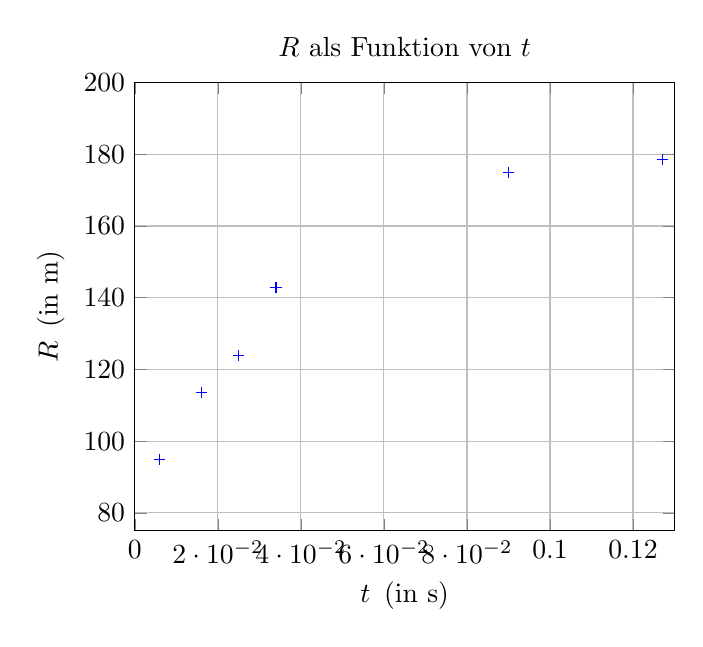
\begin{tikzpicture}
	\begin{axis}[xmin = 0, xmax = 0.13, ymin = 75, ymax = 200, grid = major, xlabel = {$t~\left(\mathrm{in~s}\right)$}, ylabel = $R~\left(\mathrm{in~m}\right)$, title ={ $R$ als Funktion von $t$} ]
%x labels  = {0,0.02,0.04,0.08,0.10,0.12}
\addplot[blue, only marks, mark = +] coordinates
{(0.006, 95.)  (0.025, 123.81) (0.016, 113.636) (0.09, 
	175.) (0.034, 142.857) (0.127, 178.571)
	};

	\end{axis}
\end{tikzpicture}
\end{figure}